\section{RS-232 – szeregowy port znakowy}
	\subsection{Co to jest?}
	Standard RS-232 został wprowadzony w 1962 r. w celu normalizacji interfejsu pomiędzy \textit{urządzeniem końcowym dla danych} (DTE - Data Terminal Equipment), a \textit{urządzeniem komunikacyjnym} (DCE - Data Communication Equipment). Na zajęciach zajmujemy się tak naprawdę zrewindowaną wersją standardu: RS-232C, wprowadzoną w 1969 roku.\\
	RS-232C umożliwia przesył danych na niewielkie odległości - do 15 metrów - oraz niewielką szybkość - do 20 kb/s - przez niesymetryczne łącze.
	\subsection{Charakterystyka interfejsu RS-232}
		Łącze szeregowe przeznaczone do asynchronicznej transmisji znakowej realizowanej zazwyczaj w trybie półdupleksowym.
		\subsubsection{Transmisja danych}
		Szeregowa asynchroniczna transmisja znakowa w trybie półdupleksowym (praktycznie tylko w tym trybie, ale mogą być inne). CIEKAWOSTKA: ma budowę dupleksową.
		\subsubsection{Rodzaje transmisji}
		\begin{itemize}
			\item Szeregowa - sekwencyjne przesyłanie bitów w ustalonej kolejności (od LSD lub MSB) po jednej linii transmisyjnej.\\
			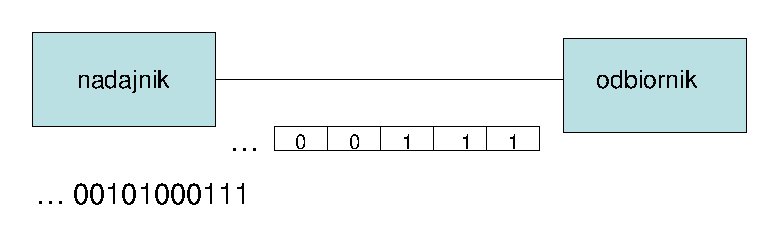
\includegraphics[width=9cm]{./wyklady/RS232_2_1.pdf}
			\item Równoległa - przesyłanie bitów słowa po przyporządkowanej każdemu bitowi linii transmisyjnej (bity przesyłane równolegle, słowa przesyłane szeregowo).\\
			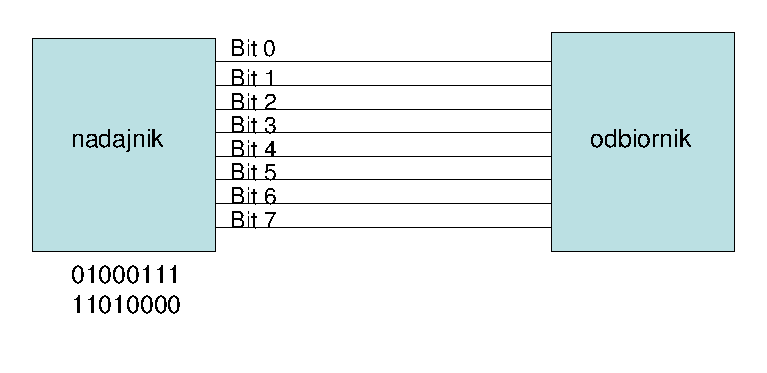
\includegraphics[width=9cm]{./wyklady/RS232_2_2.pdf}
		\end{itemize}
		\subsubsection{Definicje danych}
		\begin{itemize}
			\item "0" - 0V
			\item "1" - 12V
			\item Czas transmisji jednego bitu T - stały, nie większy niż czas propagacji.
			\item $\frac{1}{T}$ - liczba bitów przesyłana w jednostce czasu. Standardowe wartości 110, 150, 300, 600, 1200, 2400 ... [b/s]
			\item Impulsy rozeznające - sprawdzają stan bitów odebranych (następują co T, które narzuca nadawca).
		\end{itemize}
		\subsubsection{Jednostka informacyjna - znak}
		Jednostka informacji o ściśle określonym formacie. Odbiorca dysponuje impulsami próbkującymi, które rozpoznają stan sygnału (odpytują).\\
		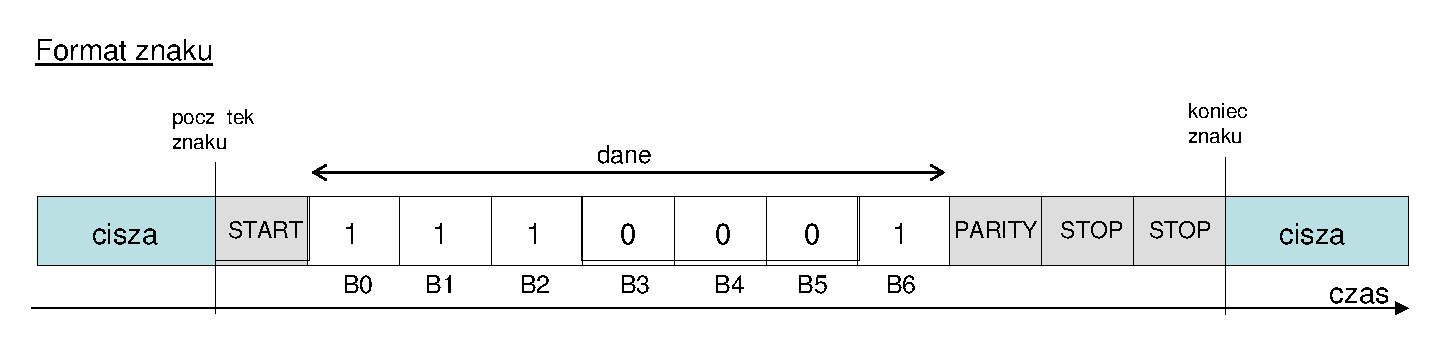
\includegraphics[width=10cm]{./wyklady/RS232_3_2.jpg}\\
		\subsubsection{Przekazywanie konfiguracji}
			Aby nadawca i odbiorca mogli się porozumieć i interpretować znaki w ten sam sposób, muszą zostać tak samo skonfigurowane. Innymi słowy, muszą posiadać ten sam takt nadawania.\\Metody:\\
			\begin{itemize}
				\item dodatkowe łącze
				\item jako element konfiguracji (wykorzystanie generatorów kwarcowych, synchronizm częstotliwościowy)
			\end{itemize}
			Nominalne położenie impulsu = ok. $\frac{1}{2}\times{T}$ - pośrodku, największe bezpieczeństwo próbkowania. Służą do tego układy korekcji fazy impulsu - liczniki, zliczają liczbę impulsów na wejściu i dają 1 na wyjściu.
		\subsubsection{Definicja znaku}
		\begin{itemize}
			\item \textbf{START} - bit kontrolny, znacznik początku (SOF - Start Of Frame) - jałowy z punktu widzenia przesyłanej informacji i służący jedynie w celu synchronizacji. START zapewnia $\frac{n}{2}$ jako stan licznika (fazy impulsu).
			\item \textbf{DANE} - 7-8 bitów (kiedyś też 5-6, obecnie już nieużywane), które są treścią znaku, począwszy od bitu najmniej znaczącego (LSB - least significant bit). Tym bitem jest B0.
			\item \textbf{PARITY} – bit kontroli poprawności znaku, służy jako zabezpieczenie informacji. Może, ale nie musi występować. Jednak decyzja o jego występowaniu ma charakter globalny - dotyczy każdego znaku w danej transmisji. Jego stan określa zasada:
			\begin{itemize}
				\item Kontrola parzystości (Even parity) - polega na sprawdzeniu liczby jedynek na polu danych i ustawieniu bitu kontrolnego na "1" w przypadku nieparzystej liczby jedynek lub na "0" w przypadku parzystej (uzupełnienie do parzystości).
				\item Kontrola nieparzystości (Odd parity) - polega na sprawdzeniu liczby zer na polu danych i ustawieniu bitu kontrolnego na "1" w przypadku nieparzystej liczby zer lub na "0" w przeciwnym przypadku.
				\item Brak kontroli (None)
			\end{itemize}
			Ten bit kontroli pozwala wykryć przekłamanie w transmisji danych pod warunkiem, ze liczba przekłamań jest nieparzysta.
			\item \textbf{STOP} – 1 lub 2 bity kontrolne, znacznik końca znaku.
		\end{itemize}
		\subsubsection{Konwencja nazewnicza rodzajów transmisji}
			[Ilość bitów danych][Rodzaj kontroli][Liczba bitów stopu]\\Przykłady:
			\begin{itemize}
				\item 7E2 - 7 bitów danych, kontrola parzystości, 2 bity stopu (10 bitów + START = 11 bitów)
				\item 8O1 - 8 bitów danych, kontrola nieparzystości, 1 bit stopu (11 bitów)
				\item 8N2 - 8 bitów danych, brak kontroli, 2 bity stopu (11 bitów)
			\end{itemize}
		\subsubsection{Rodzaje transmisji}
		\begin{itemize}
			\item \textbf{Synchroniczna} - elementy informacji wysyłane w takt zegara nadajnika. W ten sposób przesyłane są bity w ramach pojedynczej jednostki informacyjnej.
			\item \textbf{Asynchroniczna} - wysyłanie elementów informacji niesynchronizowane zegarem nadajnika. W ten sposób są wysyłane poszczególne jednostki - ich wprowadzanie nie jest sygnalizowany żadnym sygnałem, więc odstęp między nimi jest dowolny.\\
			Czas trwania bitu nazywa się \emph{odstępem jednostkowym} i oznaczamy go $t_{b}$. Jego odwrotność ($f=\frac{1}{t_{b}}$) określa szybkość transmisji w bodach, gdzie 1 [bd] = 1 [bit/s].
		\end{itemize}
		\subsubsection{Transmisja w RS-232}
		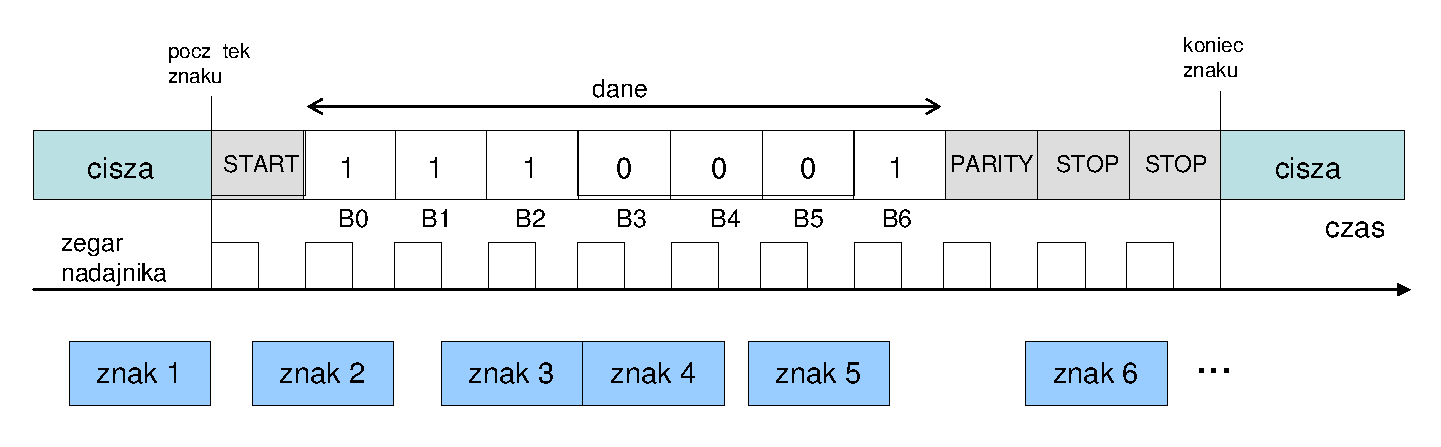
\includegraphics[width=9cm]{./wyklady/RS232_4_1.jpg}
		\begin{itemize}
			\item Synchroniczne wysyłanie bitów
			\item Asynchroniczne wysyłanie znaków
			\begin{itemize}
				\item Polega na wysyłaniu pojedynczych znaków, które mają ścisłe określony format.
				\item Brak sygnału zegarowego określającego momenty wysyłania znaków.
				\item Odstępy między znakami nieokreślone.
			\end{itemize}
		\end{itemize}
		\subsubsection{Tryby transmisji}
		\begin{itemize}
			\item \textbf{Simpleksowa} - jednokierunkowa, z nadajnika do odbiornika.
			\item \textbf{Półdupleksowa} (HDX) - dwukierunkowa, niejednoczesna (w danej chwili czasu jedno urządzenia jest nadajnikiem, a drugie odbiornikiem). Zakłada istnienie tylko jednej linii transmisyjnej. Wymaga konfiguracji (informacja, kto kiedy nadaje).
			\item \textbf{Dupleksowa} (FDX) - dwukierunkowa, jednoczesna (w danej chwili czasu oba urządzenia mogą spełniać rolę nadajnika lub odbiornika). Brak konieczności sprawdzania czy łącze jest wolne oraz mechanizmu rezerwacji łącza.
		\end{itemize}
	\subsection{Komunikacja DTE-DCE - sygnały w porcie RS-232}
	Komunikacja dwóch stacji DTE przez komutowane łącze telefoniczne.\\
	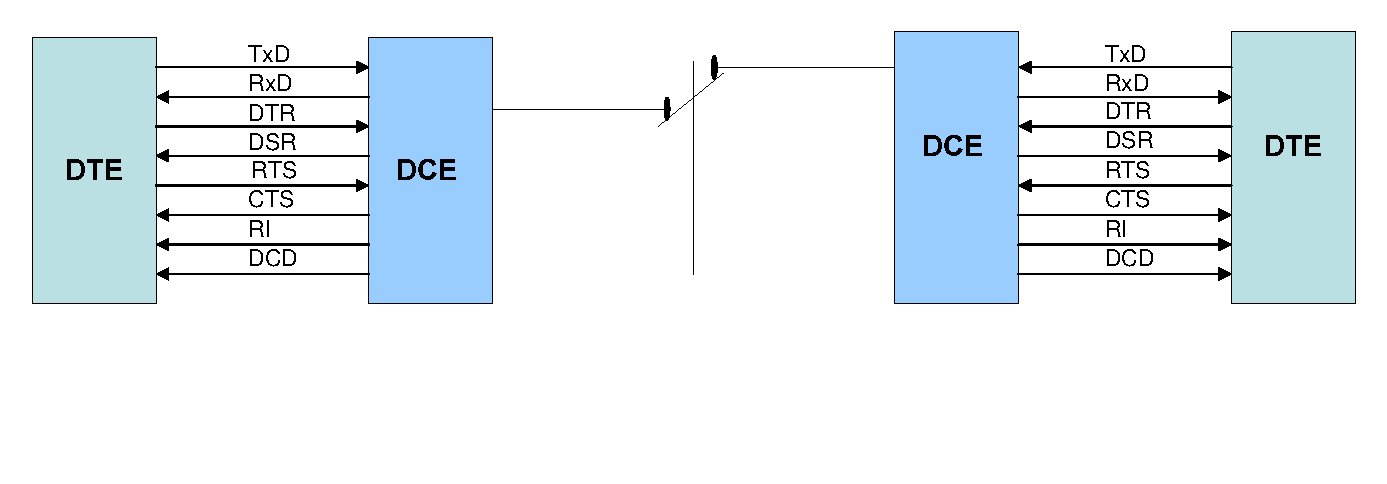
\includegraphics[width=12cm]{./wyklady/RS232_6_1.pdf}\\
	\begin{table}[h]
		\begin{tabular}{|c|c|c|c|c|}
			\hline
			\multicolumn{5}{|c|}{\textbf{Urządzenia}}                        \\ \hline
			\multicolumn{1}{|c|}{DTE} & \multicolumn{2}{|c|}{Data Terminal Equipment}      & \multicolumn{2}{|c|}{Komputer}           \\ \hline
			\multicolumn{1}{|c|}{DCE} & \multicolumn{2}{|c|}{Data Communication Equipment} & \multicolumn{2}{|c|}{Modem}              \\ \hline
			\multicolumn{5}{|c|}{\textbf{Linie} (sygnały)}                   \\ \hline
			\textbf{Skrót} & \textbf{Nazwa}	   & \textbf{Znaczenie} & \textbf{Przeznaczenie} & \textbf{Kierunek} \\ \hline
			TxD & Transmitted Data             & Dane nadawane      & Linia danych		& Wyjście	\\ \hline
			RxD & Received Data                & Dane odbierane     & Linia danych		& Wejście	\\ \hline
			DTR & Data Terminal Ready          & Gotowość DTE       & Linia kontrolna	& Wyjście	\\ \hline
			DSR & Data Set Ready               & Gotowość DCE       & Linia kontrolna	& Wejście	\\ \hline
			RTS & Request to Send              & Żądanie nadawania  & Linia kontrolna	& Wyjście	\\ \hline
			CTS & Clear To Send                & Zgoda na nadawanie & Linia kontrolna	& Wejście	\\ \hline
			RI  & Ring Indicator               & Wskaźnik wywołania & Linia kontrolna   & Wejście	\\ \hline
			DCD & Data Carrier Detected        & Wykrycie nośnej    & Linia kontrolna   & Wejście	\\ \hline
			SG  & Signal Ground                & Masa sygnałowa     & Masa				& ------	\\ \hline
		\end{tabular}
	\end{table}
		\subsubsection{Fazy pracy układu}
		\begin{itemize}
			\item Tryb nawiązywania połączenia
			\item Tryb transmisji danych (wtedy nas interesują dupleksy i inne)
		\end{itemize}
		\subsubsection{Linie w złączu RS-232}
		\begin{itemize}
			\item Linie danych: TxD, RxD
			\item Linie kontrolne: DTR, DSR, RTS, CTS, RI, DCD
		\end{itemize}
	\subsection{Połączenie bezmodemowe DTE-DTE}
	Przykład połączenia dla transmisji dupleksowej.\\
	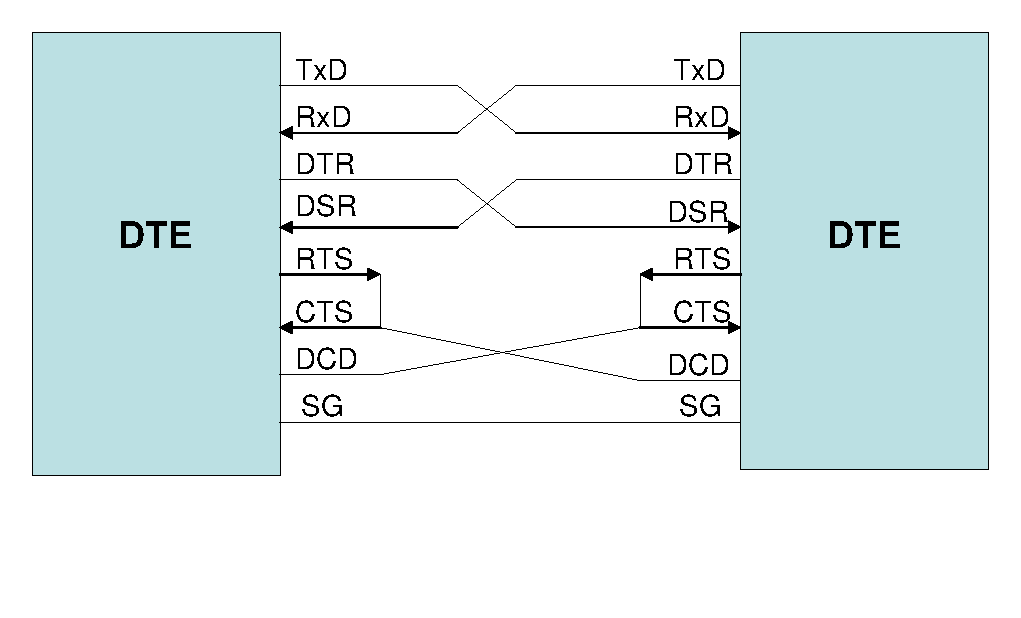
\includegraphics[width=9cm]{./wyklady/RS232_7_1.pdf}
	\begin{itemize}
		\item PG, SG - masa
		\item TxD, RxD - dane
		\item RTS, CTS, DCD, DSR, DTR - sterowanie
	\end{itemize}
	\subsection{Kontrola transmisji: handshake i protokół XON/XOFF}
		\subsubsection{Handshake}
		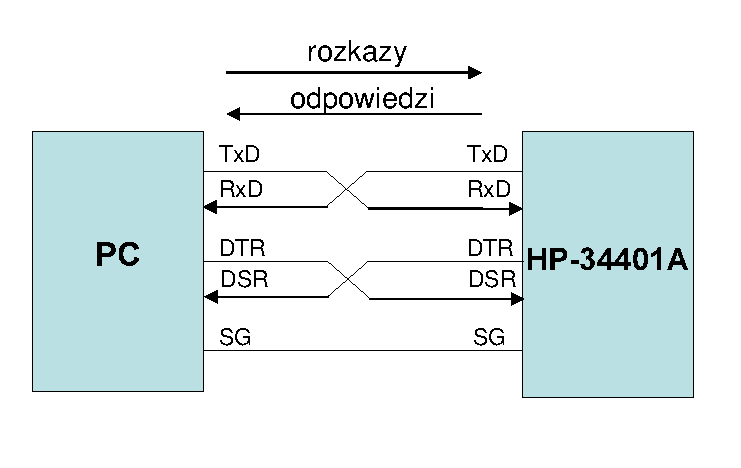
\includegraphics[width=9cm]{./wyklady/RS232_9_1.pdf}
		\begin{itemize}
			\item DTR = 1 - zgoda na nadawanie
			\item DTR = 0 - brak zgody na nadawanie
			\item DTR informuje, czy bufor jest zapełniony. DSR sprawdza go u partnera przed wysłaniem dalszych danych.
			\item Analogiczna sytuacja, kiedy podłączone są RTS i CTS zamiast DTR i DSR. RTS wystawia informację, CTS sprawdza.
		\end{itemize}
		\subsubsection{Protokół XON/XOFF}
		Występuje przy wymianie informacji w trybie dupleksowym. Umożliwia blokowanie i odblokowywanie transmisji danych. Np. drukarka - gdy skończy się papier w trakcie drukowania, przesył jest blokowany, Gdy użytkownik uzupełni papier, transmisja jest wznawiana. Taki protokół XON/OFF nazywany jest programowym (software XON/OFF). {\small Rozwiązanie hardware to transmisja półdupleksowa za pośrednictwem sygnałów w kanale wtórnym.}\\
		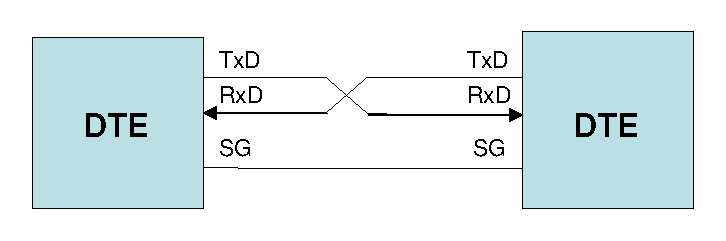
\includegraphics[width=9cm]{./wyklady/RS232_9_2.pdf}
		\begin{itemize}
			\item XON – ASCII 19 (CTRL-S)
			\item XOFF – ASCII 17 (CTRL-Q)
		\end{itemize}
	\subsection{Parametry elektryczne sygnałów}
	Poniżej przestawiono schemat "obwodu stykowego" złożonego ze źródła sygnału, toru transmisyjnego i odbiornika. Parametry zdefiniowano przy założeniu, że szybkość transmisji nie przekracza 20 kbd.
	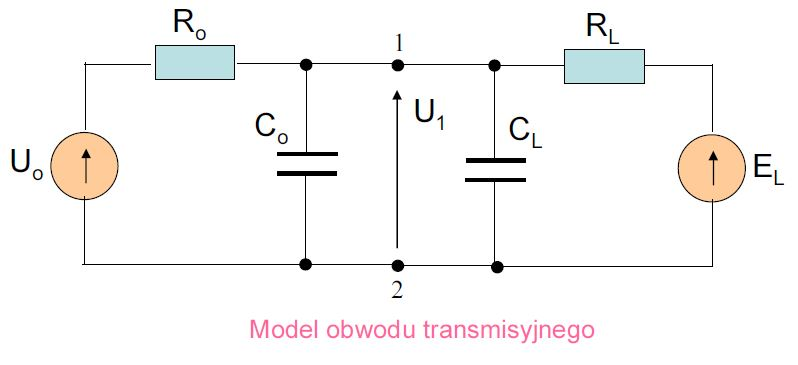
\includegraphics[width=9cm]{./wyklady/RS232_10_1.jpg}\\
	Na rysunku powyżej: kiloomy oraz mikrosekundy.\\
	Wada: jest to obwód represyjny, da się go silnie zakłócić poprzez różnicę potencjałów pomiędzy masami.
	\subsection{Standardy RS-423, RS-422, RS-485}
	Niesymetryczna przesyłanie danych w RS-232C ogranicza szybkość i odległość transmisji, a ponadto nie jest zabezpieczone przed zakłóceniami zewnętrznymi. Aby to polepszyć wymyślono inne standardy.
		\subsubsection{RS-423A}
		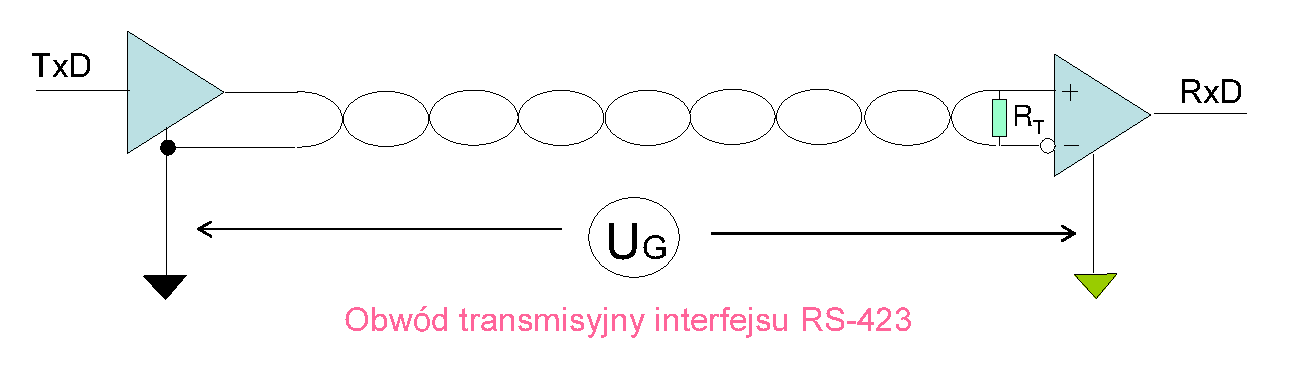
\includegraphics[width=9cm]{./wyklady/RS232_12_1.pdf}
		\begin{itemize}
			\item szybkość do 100 kbd (przy zasięgu do 30 m)
			\item zasięg do 1200 m (przy szybkosci do 3 kbd)
		\end{itemize}
		Standard RS-423A określa elektryczną charakterystykę napięciowego obwodu transmisyjnego złożonego z niesymetrycznego nadajnika oraz symetrycznego (różnicowego) odbiornika. Takie obwody stosuje się do przesyłania sygnałów binarnych pomiędzy DTE i DCE, które reprezentują dane lub funkcje sterujące.\\
		Zastosowanie różnicowego obciążenia pozwala na znaczne zmniejszenie wpływu napięcia wspólnego $U_{G}$ powstałego na wskutek różnicy potencjałów masy nadajnika i odbiornika, jak również przesłuchów między nimi.\\
		Standard wymaga aby dla każdego kierunku transmisji istniał przynajmniej jeden niezależny przewód powrotny.\\
		Typowa prędkość wynosi 100 kb/s przy odległości do 30 m.
		\subsubsection{RS-422A}
		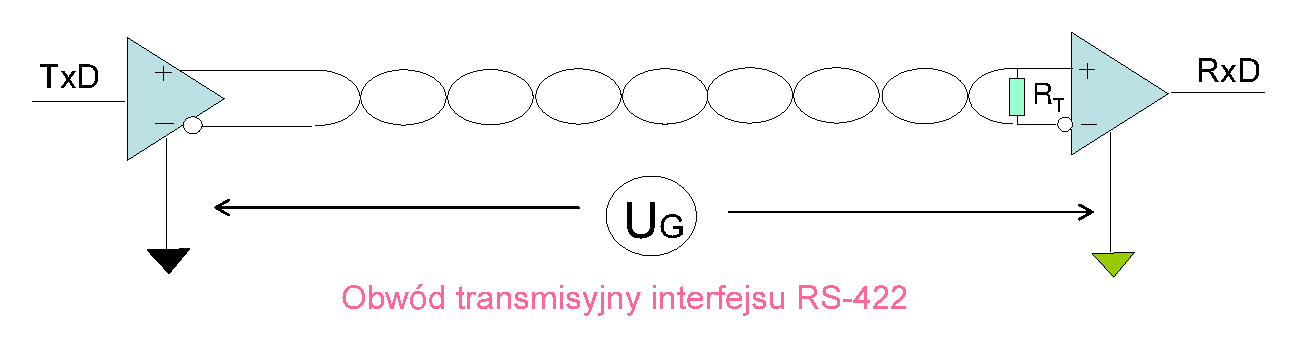
\includegraphics[width=9cm]{./wyklady/RS232_12_2.pdf}
		\begin{itemize}
			\item szybkość do 10 Mbd (przy zasięgu do 100 m)
			\item zasięg do 1200 m (przy szybkości 100 kbd)
		\end{itemize}
		Wykorzystuje pełną symetryzację łącza, zapewnia szybka transmisję w obecności zakłóceń. Standardy RS-423 oraz RS-485 określają symetryczny, zrównoważony system transmisji danych złożony z:
		\begin{itemize}
			\item różnicowego nadajnika
			\item dwuprzewodowego zrównoważonego toru przesyłowego
			\item odbiornika o różnicowym obwodzie wejściowym.
		\end{itemize}
		Standard RS-422A nie wprowadza ograniczeń na minimalną i maksymalną częstotliwość, a jedynie na zależność między szybkością zmian sygnału, a czasem trwania bitu.
		\subsubsection{RS-485A}
		Standard RS-485A jest rozwinięciem RS-422. Łącze RS-485A jest również zrównoważone i symetryczne, przy czym dopuszcza się nie tylko wiele odbiorników, ale i wiele nadajników podłączonych do jednej linii. Nadajniki muszą być trójstanowe.\\
		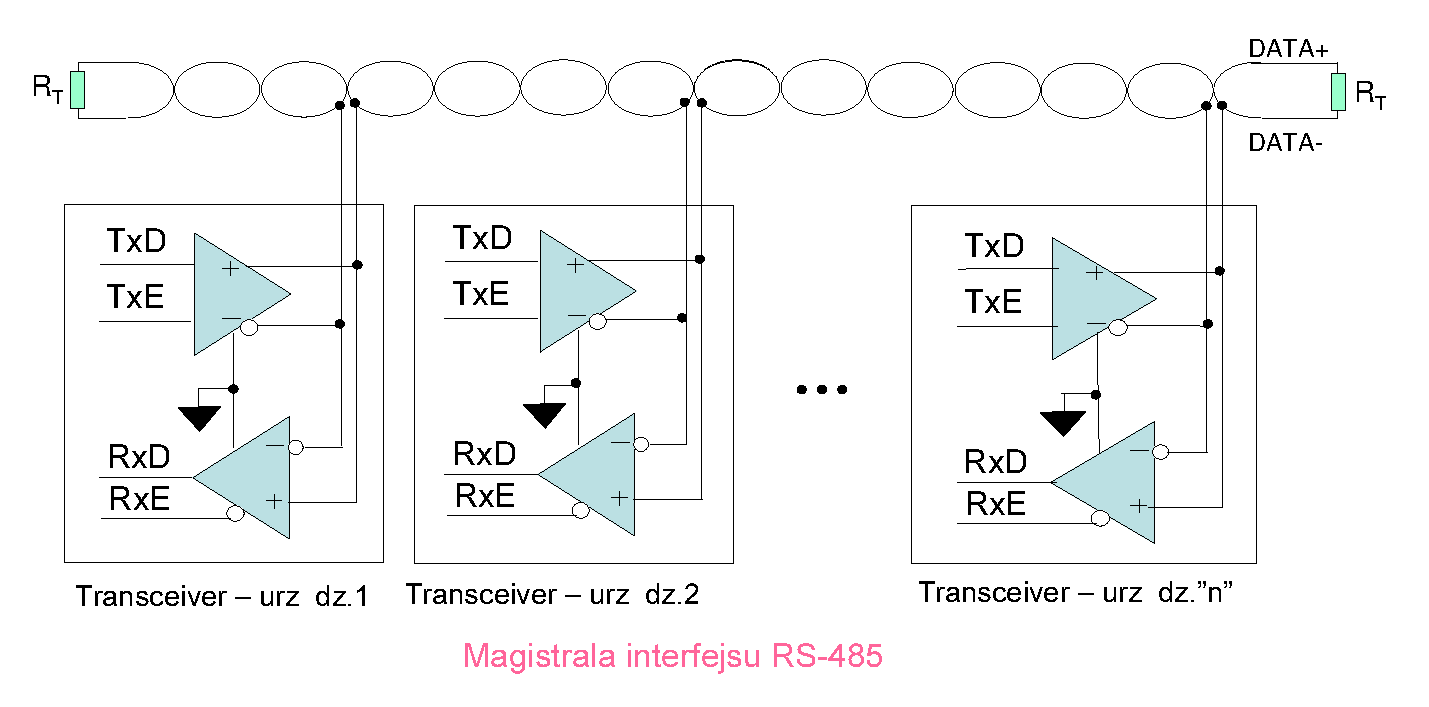
\includegraphics[width=10cm]{./wyklady/RS232_13_1.jpg}
	\subsection{Systemy komunikacyjne oparte na łączu znakowym}
		\subsubsection{System oparty na szeregowym łączu znakowym}
		Podłączenie urządzenia RS-232 do portu COM z pom. int. RS-485\\
		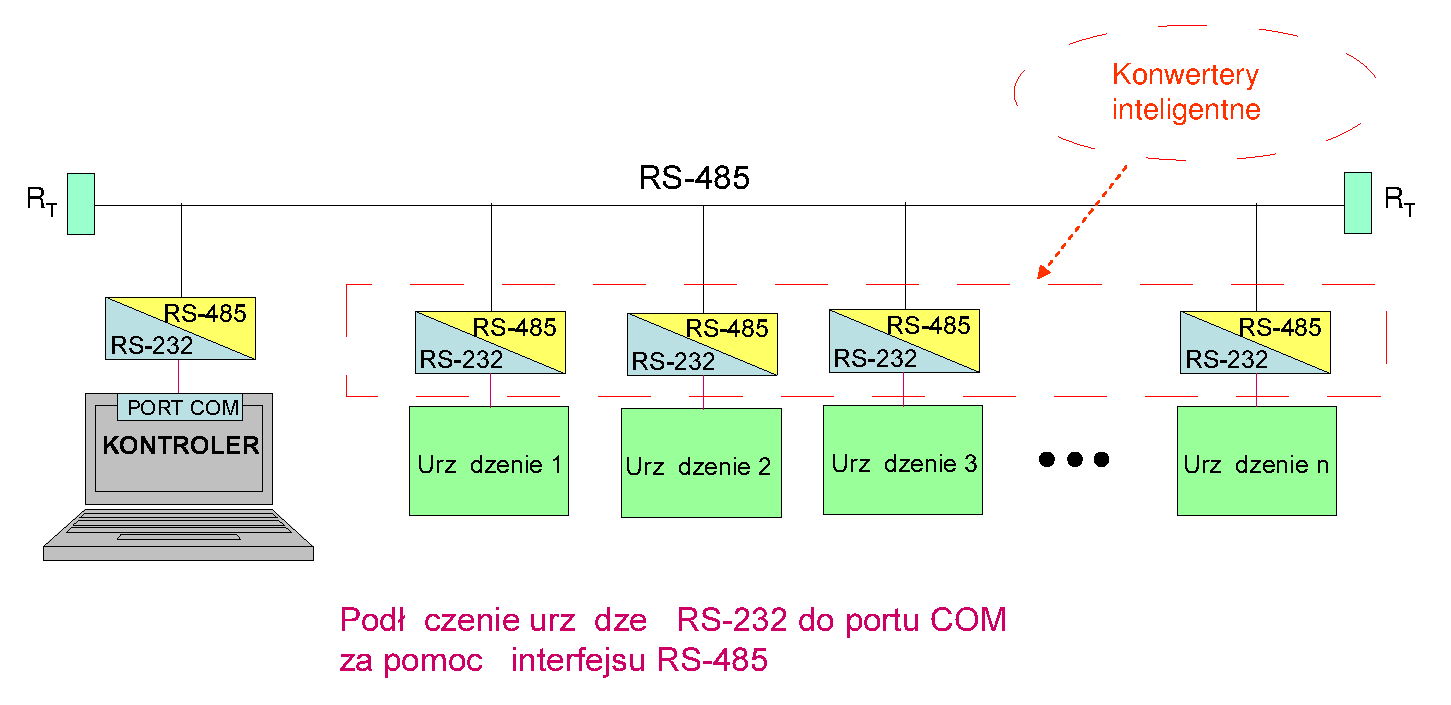
\includegraphics[width=9cm]{./wyklady/RS232_14_1.jpg}\\
		R\tiny T\normalsize - Rezystory zabezpieczające przed niekorzystnym odbiciem fali (tzw. Terminatory).\\
		\textbf{Problem}: dostęp do magistrali kontrolera i urządzeń systemu\\
		\textbf{Rozwiązanie}: Implementacja protokołu komunikacyjnego (warstwa łącza danych). Komputer zarządza innymi urządzeniami w całym systemie. Do zbudowania tego wystarczają proste przejściówki do zmian sygnałów.\\
		\textbf{Komunikacja}:
		\begin{itemize}
			\item Selekcja urządzenia kontrolującego (master) - generuje on rozgłoszenie (broadcast) do wszystkich urządzeń i zbiera dane.
			\item Selekcja urządzenia odbierającego - konieczna gdy wiele urządzeń chce przesłać odpowiedź do mastera, co może powodować konflikt.
			\begin{itemize}
				\item nadanie identyfikatorów (adresacja urządzeń)
				\item zastosowanie przejściówek - są inteligentne i odpowiadają za dostęp do urządzenia.
			\end{itemize}
		\end{itemize}
		\subsubsection{System oparty na łączu znakowym}
		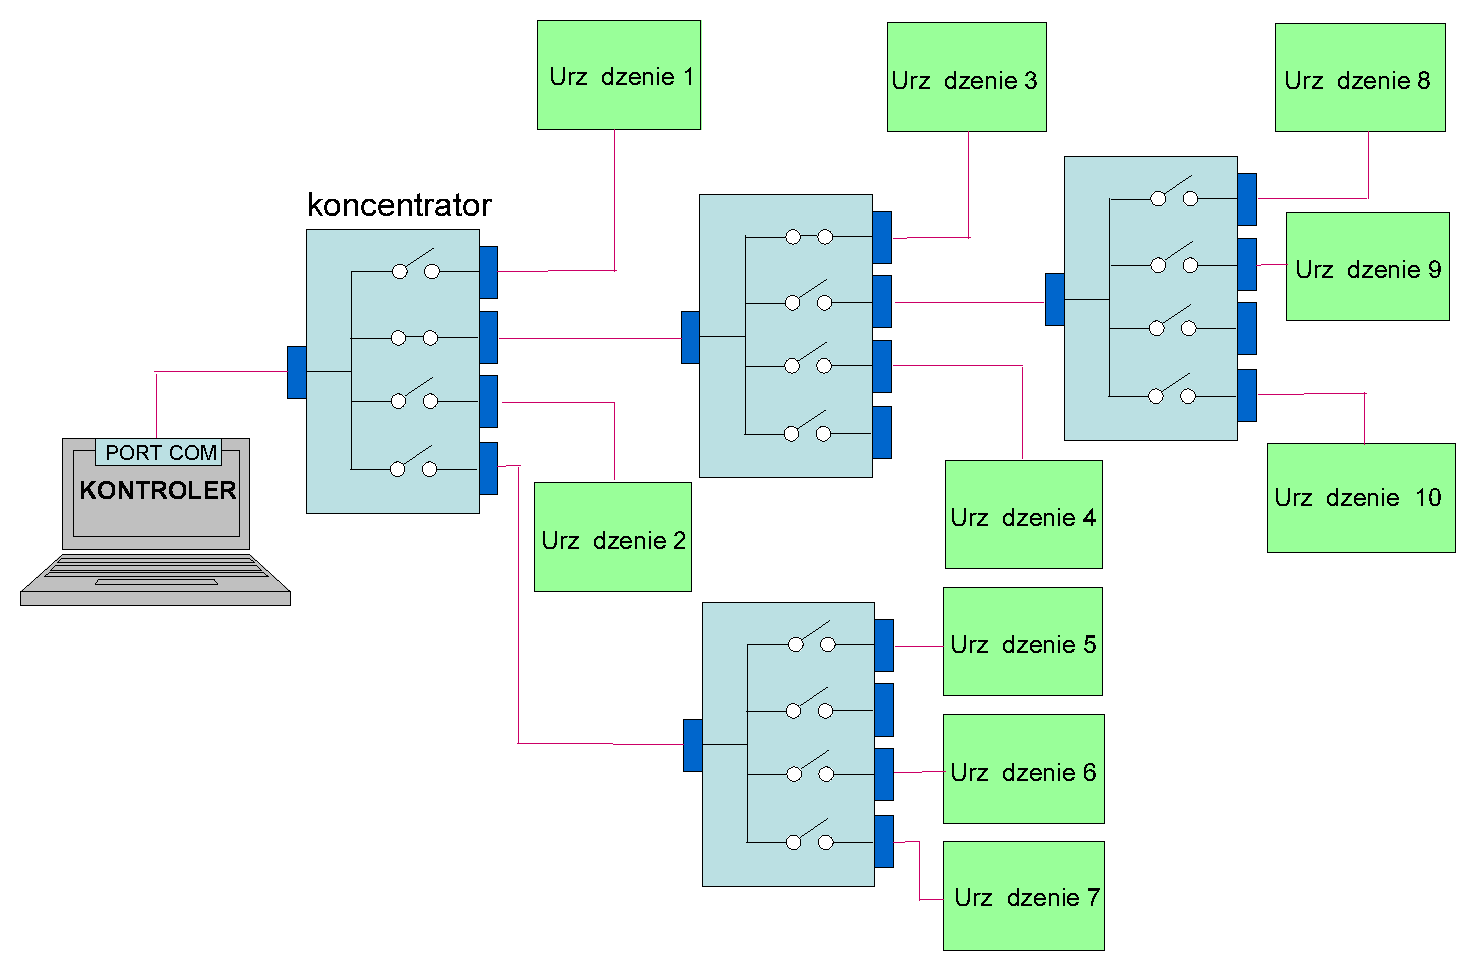
\includegraphics[width=10cm]{./wyklady/RS232_15_1.jpg}\\
		Koncentrator zawiera 4 klucze portu RS. Dostęp jest tylko do jednego wyjścia naraz.\\
		\textbf{Kaskadowe połączenie} - przełącznik podłączony do przełącznika. Pojawia się problem wyboru drogi do urządzenia, która musi być znana. Koncentratory muszą mieć informacje o \textbf{mapie urządzeń}.
	\subsection{System MODBUS}
		Interfejs MODBUS został opracowany w firmie Modicon i jest przyjętym standardem w dla asynchronicznej, znakowej wymiany informacji pomiędzy urządzeniami systemów pomiarowo-kontrolnych.
		\subsubsection{Charakterystyka}
			\begin{itemize}
				\item Reguła dostępu do łącza na zasadzie Master-Slave. 
				\item Zabezpieczenie przesyłanych komunikatów przed błędami
				\item Potwierdzenie wykonania rozkazów zdalnych i sygnalizacja błędów
				\item Mechanizmy zabezpieczające przed zawieszeniem systemu
				\item Wykorzystanie asynchronicznej transmisji znakowej zgodnej z RS-232C
			\end{itemize}
		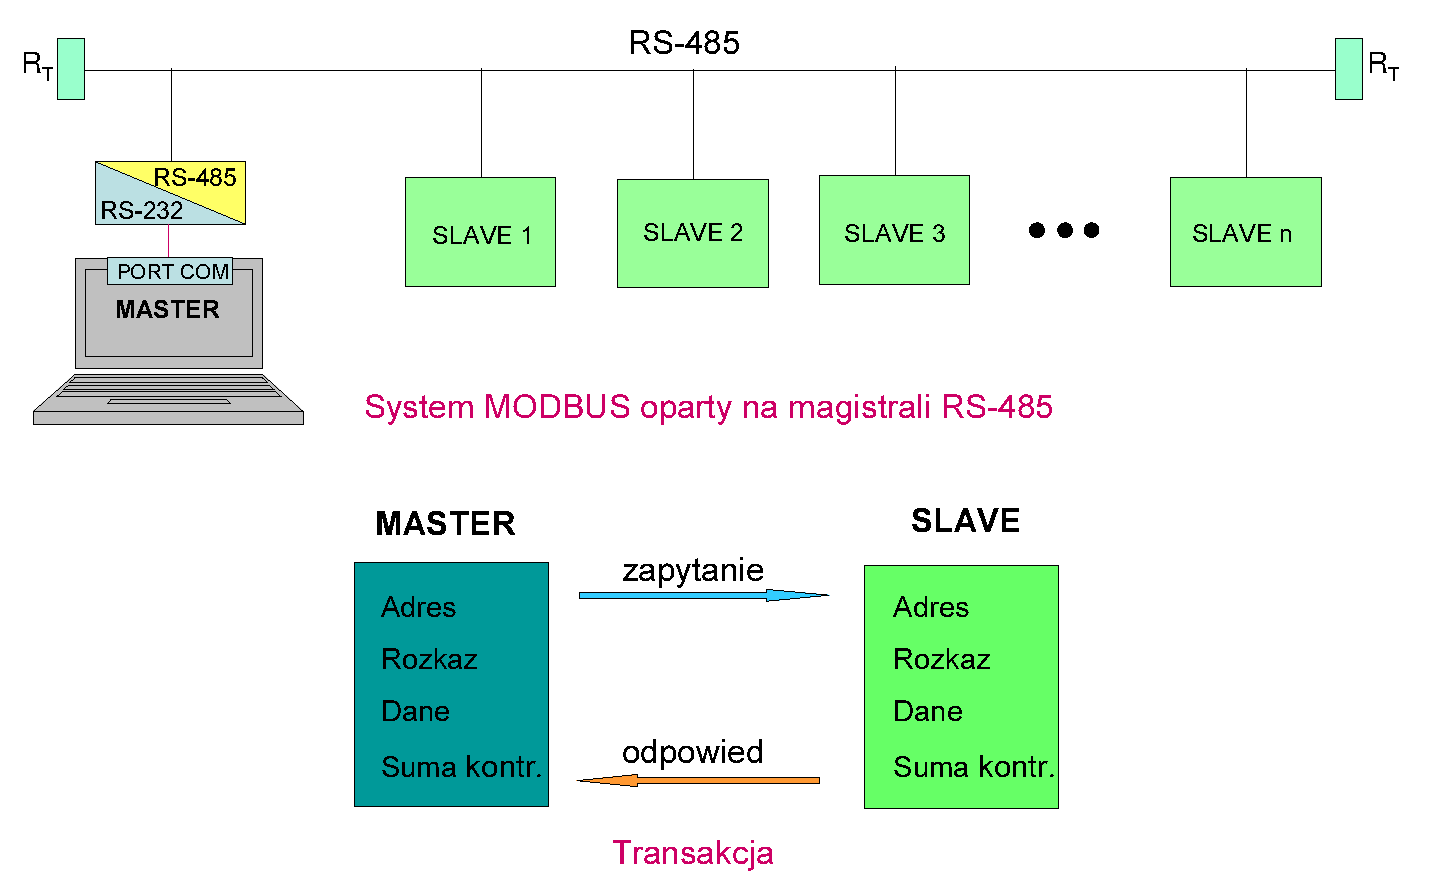
\includegraphics[width=9cm]{./wyklady/RS232_16_1.jpg}\\
		\subsubsection{Transakcja}
		Jedno urządzenie może inicjować transakcje (master), a pozostałe (slave) odpowiadają jedynie na zapytania mastera. Transakcja składa się z polecenia (query) wysyłanego z master do slave oraz z odpowiedzi (response) przesyłanej ze slave do master. Odpowiedź zawiera dane żądane przez master lub potwierdzenie realizacji jego połączenia. Wykrycie końca kończy fazę w której następuje przekazanie łącza masterowi.\\
		\subsubsection{Format wiadomości}
		Dotyczy zarówno poleceń jednostki nadrzędnej, jak i odpowiedzi podrzędnych.
		\begin{itemize}
			\item Adres
			\item Kod funkcji reprezentujący rozkaz, pierwszy bit rozkazu oznacza jego rodzaj. 0 - normalny, 1 - szczególny.
			\item Dane
			\item Kontrola błędów (dla pracy w warunkach przemysłowych)
		\end{itemize}
		W przypadku odpowiedzi odpowiednio w polach znajdują się:
		\begin{itemize}
			\item Adres (swój, slave'a, do kontroli poprawności)
			\item Pole potwierdzenia realizacji rozkazu
			\item Dane żądane przez master
			\item Kontrola błędów
		\end{itemize}
		\subsubsection{Rodzaje transakcji}
			\begin{itemize}
				\item \textbf{Adresowana} - przeznaczona dla pojedynczej jednostki slave
				\item \textbf{Rozgłoszeniowa} (broadcast) - wysyłana do wszystkich jednostek podrzędnych. Na ten rodzaj polecenia jednostki nie przesyłają odpowiedzi.
			\end{itemize}
		\subsubsection{Rodzaje odpowiedzi}
			\begin{itemize}
				\item \textbf{Normalna} - w przypadku poprawnego wykonania polecenia.
				\item \textbf{Szczególna} - jeżeli slave wykryje błąd przy odbiorze wiadomości lub nie jest w stanie wykonać polecenia, to przygotowuje specjalny komunikat o wystąpieniu błędu i przesyła jako odpowiedź. W przypadku tej wiadomości jest ona \textbf{powiększona} o 128 - miejsce na kod błędu.
			\end{itemize}
		\subsubsection{Parametry protokołu}
			\begin{itemize}
				\item Reguła dostępu do łącza: Master-Slave
				\item Zakres adresów: 1 - 247 (identyfikatory slave'ów)
				\item Adres rozgłoszeniowy: 0, rozpoznawany przez wszystkie slave'y
				\item Kontrola błędów: LRC/CRC, ograniczenie czasowe odpowiedzi
				\item Wymagana ciągłość przesyłania znaków w ramce
			\end{itemize}
		\subsubsection{Ramka w systemie MODBUS}
			W systemie MODBUS wiadomości są zorganizowane w ramki o określonym początku i końcu. Umożliwia do odbiornikowi odrzucenie ramek niekompletnych i sygnalizację błędów.
		\subsubsection{Rodzaje transmisji ramek}
			\begin{itemize}
				\item ASCII
				\item RTU
			\end{itemize}
		\subsubsection{Ramka w trybie ASCII}
			Każdy bajt wiadomości przesyłany jest w postaci dwóch znaków ASCII. Zaletą tego rozwiązania jest to, że pozwala na długie odstępy między znakami (1 s) bez powodowania błędów.\\\\\textbf{Format znaku}\\
			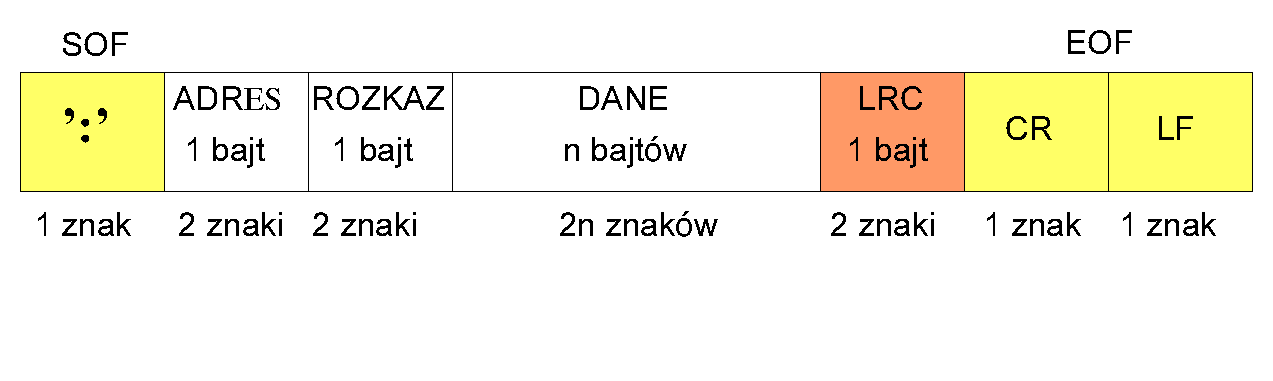
\includegraphics[width=10cm]{./wyklady/RS232_18_1.pdf}
			\begin{itemize}
				\item System kodowania: heksadecymalny, znaki ASCII 0-9, A-F. Jeden znak heksadecymalny zawarty jest w każdym znaku ASCII wiadomości.
				\item Jednostka informacyjna: ograniczona znakami start (na początku) i stop (na końcu), 10-bitowa.
				\item Znacznikiem początku ramki jest znak dwukropka (":" - ASCII 3Ah).
				\item Dopuszczalne znaki dla pozostałych pól (poza znacznikiem końca ramki) to 0-9, A-F.
				\item Pole funkcji: dwa znaki w trybie ASCII
				\item Podsumowując: wykorzystujemy 2 znaki heksadecymalne do przesyłu 1go znaku ASCII. Dzielimy ten na dwie części i przesyłamy w dwóch pakietach po 10 bitów.
				\item Urządzenie po wykryciu znacznika początku sprawdza czy pole adresowe zawiera jego własny adres. Jeżeli tak, to odczytuje zawartość pola funkcji i pola danych.
				\item Pole kontrolne LRC (1-bitowe) zabezpiecza część informacyjną. Sumuje cześć informacyjną bajtu i uzupełnia do 2.
				\item Ramka kończy się przesłaniem dwóch znaków: CR i LF.
				\item Ramkę kończy przerwa czasowa trwająca co najmniej $3.5\times$(długości znaku)
				\item Ramki muszą być przesyłane w postaci ciągłej, tzn. odstęp między kolejnymi znakami tworzącymi ramkę nie może być większy niż $1.5\times$(długości znaku).
			\end{itemize}
			Stosowane jest zabezpieczenie części informacyjnej ramki kodem LRC (Longitudinal Redundancy Check).
		\subsubsection{Ramka w trybie RTU}
			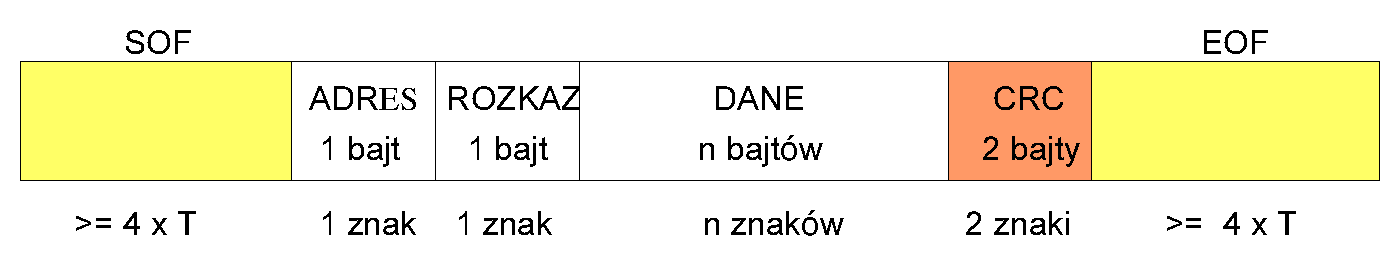
\includegraphics[width=10cm]{./wyklady/RS232_18_2.pdf}\\
			W trybie RTU wiadomości zaczynają się odstępem czasowym trwającym minimum $3.5\times$(\emph{czas trwania pojedynczego znaku}), w którym panuje cisza na łączu (można to zrealizować np. przez odmierzanie czasu trwania znaku przy zadanej na łączu szybkości bodowej).
			\begin{itemize}
				\item Pierwszym polem informacyjnym jest adres urządzenia
				\item Dopuszczalne znaki w ramach pól ramki: 0-9, A-F
				\item Zakres kodów operacji: 1 - 255
				\item Urządzenia stale monitorują magistralę. Jak adres odebrany w wiadomości zgadza się z ich własnym, to lecą dalej.
				\item Ramkę kończy przerwa czasowa trwająca co najmniej $3.5\times$(długości znaku)
				\item W przypadku gdy nowa wiadomość pojawia się przed upływem niezbędnej przerwy to będzie ona potraktowana jako kontynuacja poprzedniej wiadomości. Doprowadzi to do błędu sumy kontrolnej.
				\item Ramki muszą być przesyłane w postaci ciągłej, tzn. odstęp między kolejnymi znakami tworzącymi ramkę nie może być większy niż $1.5\times$(długości znaku).
				\item Przekroczenie odstępu powoduje uznanie ramki za niekompletną i błędną.
				\item Kontrola danych typu CRC - 2-bajtowe, silniejsze niż LRC.
			\end{itemize}
		\subsubsection{Warstwa fizyczna}
		\begin{itemize}
			\item Asynchroniczna transmisja znakowa
			\item Formaty znaków
			\begin{itemize}
				\item Tryb ASCII: 7E1, 7O1, 7N2
				\item Tryb RTU: 8E1, 8O1, 8N2
			\end{itemize}
			\item Szybkość: od 1200 bd do 19200 bd
			\item Rodzaj łącza:
			\begin{itemize}
				\item Magistrala RS-485
				\item Multipleksowany RS-232
			\end{itemize}
			\item Rodzaj transmisji (zależny od łącza):
			\begin{itemize}
				\item różnicowa dla RS-485
				\item odniesiona do masy dla RS-232
			\end{itemize}
		\end{itemize}
	\subsection{Kontroler RS-232 w komputerze PC}